%
%  Erik Olsen
%
\documentclass[12pt,fullpage]{article}
\usepackage{fullpage}                                        % use all of the page for text 
\usepackage{psfrag}                                          % LaTeX graphics tool
\usepackage{pslatex}                                         % avoids the default cmr font
\usepackage{graphicx}                                        % graphics package 
\usepackage{epsfig}                                          % figures
\usepackage{epsfig} 
\usepackage{hyperref}
\usepackage{color}

\begin{document}

\noindent
{\bf Generalized Pareto distribution} (from \color{blue}\url{http://www.math.wm.edu/~leemis/chart/UDR/UDR.html}\color{black})

\noindent
The shorthand $X \sim$ generalized Pareto$(\delta,\kappa,\gamma)$ is used to indicate that the
random variable $X$ has the generalized Pareto distribution with shape parameters
$\delta, \kappa$ and $\gamma$.
A generalized Pareto random variable $X$ has probability density function 
$$
f(x) = \left(\gamma + \frac{\kappa}{x + \delta}\right)\left(1+ x / \delta\right) ^ {- \kappa} e ^ {- \gamma \kern 0.08em x}      \qquad \qquad \delta > 0;\ \  \gamma\geq 0;\ \  \kappa \geq - \delta \kern 0.08 em \gamma
$$
for $x > 0$.  The probability density function with two different parameter combinations
is illustrated below.
\begin{figure}[h!]
\begin{center}
\psfrag{lab1}{$\delta \kern -0.08 em = \kern -0.08 em  1,\, \gamma \kern -0.08 em  = \kern -0.08 em  1,\, \kappa \kern -0.08 em  = \kern -0.08 em  1$}
\psfrag{lab2}{$\delta \kern -0.08 em  = \kern -0.08 em  10,\, \gamma \kern -0.08 em  = \kern -0.08 em  .5,\, \kappa \kern -0.08 em  = \kern -0.08 em  1$}
\psfrag{labx}{$x$}
\psfrag{labf}{$f(x)$}
\includegraphics[width=3.2in]{GeneralizedparetoPlot.ps}
\end{center}
\end{figure}

\noindent
The cumulative distribution function on the support of $X$ is
$$
F(x) = P(X \le x) =1- e ^ {- \gamma \kern 0.08em x}\,\left(1 + x/ \delta\right)^{-\kappa}  \qquad \qquad x > 0.
$$
The survivor function on the support of $X$ is
$$
S(x) = P(X \ge x) = e ^ {- \gamma \kern 0.08em x}\,\left(1 + x/\delta\right) ^ {- \kappa}\qquad \qquad x > 0.
$$
The hazard function on the support of $X$ is
$$
h(x) =\frac{f(x)} {S(x)}= \gamma + \frac{\kappa}{x + \delta} \qquad \qquad x > 0.
$$
The cumulative hazard function on the support of $X$ is
$$
H(x) =  -\ln S(x) = \gamma \kern 0.08 em x + \kappa \ln(1 + x/ \delta) \qquad \qquad x > 0.
$$
The moment generating function and characteristic function of $X$, as well as the population mean, variance, skewness and kurtosis of $X$, are mathematically intractable.

%\vspace{0.1in}
%\newpage
%\noindent
%{\bf APPL verification:}
%The APPL statements
%\begin{verbatim}
%assume(g > 0);
%assume(d >= 0);
%assume(k >= -d * g);
%X := [[x -> (g + k / (x + d)) * exp(-g * x) / ((1 + x / d) ^ k)],
%      [0, infinity], ["Continuous", "PDF"]];
%CDF(X);
%SF(X);
%HF(X);
%CHF(X);
%Mean(X);
%Variance(X);
%Skewness(X);
%Kurtosis(X);
%MGF(X);
%\end{verbatim}
%verify the cumulative distribution function, survivor function, hazard function,
%cumulative hazard function, population mean, variance, skewness, kurtosis, and
%moment generating function.
\end{document}
